
%(BEGIN_QUESTION)
% Copyright 2006, Tony R. Kuphaldt, released under the Creative Commons Attribution License (v 1.0)
% This means you may do almost anything with this work of mine, so long as you give me proper credit

A primitive kind of thermometer is called a {\it Galileo thermometer}, and it looks something like this:

$$\includegraphics[width=15.5cm]{i00281x01.eps}$$

Ambient temperature is indicated by the whichever ball is floating mid-way inside the liquid container.  In this case, the indicated temperature is 72$^{o}$ F.  Explain the operating principle of this thermometer.

\vskip 10pt

A simple form of {\it densitometer} is used to measure the concentration of anti-freeze additive in automotive engine coolant.  It somewhat resembles a Galileo thermometer, and it is read the same way (by seeing how many of the balls float):

$$\includegraphics[width=15.5cm]{i00281x02.eps}$$

Explain how this instrument works, and how its operating principle relates to that of the Galileo thermometer.

\underbar{file i00281}
%(END_QUESTION)





%(BEGIN_ANSWER)

A Galileo thermometer works on the principle of liquid density changing with temperature.  As the liquid density changes with ambient temperature, different balls will achieve neutral buoyancy.

\vskip 10pt

For the densitometer, more balls will float as the fluid becomes denser.  This equates to a ``stronger'' concentration of antifreeze in the coolant mixture.

%(END_ANSWER)





%(BEGIN_NOTES)

A Galileo thermometer works on the principle of liquid density changing with temperature.  The balls are fixed-density, and each one has a slightly different density than the others.  As the liquid density changes with ambient temperature, different balls will achieve neutral buoyancy (density equal to that of the surrounding liquid), thus indicating the ambient temperature.

Likewise, the ball-type densitometer uses balls of differing density.

%INDEX% Measurement, density: ball-type densitometer
%INDEX% Measurement, temperature: Galileo thermometer

%(END_NOTES)


